\pfMakeSplashHeader[
  image = oneshot,
  title = The Rats of Nhime,
  headerHeight = -7cm,
  textBodyHeight = 6cm
]

\chapter{The Rats of Nhime}

This island is a lush tropical paradise, filled with jutting bluffs of volcanic stone and white-sand beaches. The towering palm trees obscure the source of lively bird chatter, and the sound of snorting and squealing in the distance betrays the wildlife. The humidity here is dense, and the sweet smell of the purple flowers on vines lining the underbrush fill your senses.

\begin{multicols}{2}

  \section{Setup}
  The following sections detail the setup for the adventure and everything you should know before starting. There are specific headings provided to give you, the GM, a clear idea of how to steer this adventure.

  \subsection{Plot Hook}
  The serenity of the locale is contrasted sharply by the bloody goblins lying dead in the path. A quick check indicates no external source. Up the path, they meet a village elder at the town square by the well, casting magic upon it to purify the contents of a bucket. She offers coin to cleanse the well and save the town.

  \begin{minipage}[t]{.15\textwidth}
    
\includegraphics[width=3in]{book/img/Swarm_Voice}
  \end{minipage}

  \subsection{Big Bad}
  Corrupted Swarm voice.

  \subsection{Relevant NPCs}
  Goblin village elder has info on the poison that started shortly after a giant monster flew through the sky. It circled this island once before a blinding red lightning bolt came down and impacted somewhere deeper in the island.

  The women and children have been vacated to a remote location.

  A child has come away from them to find their father. This child can be interacted with (if time permits).

  \subsection{Rivals}
  A group of 3 monster hunters challenge the group to be the first to find the source of the poisoned water source. They roll up at the same time as the PC's and introduce themselves. They are from the same order and heard about how their group did not foil the prophecy. They were sent to clean up after PC's mess.

  \subsection{Challenges}
  Four traps on the way and 2 in the miniboss fight.

  \subsection{Key Locations}
  \begin{itemize}
    \item Goblin town.
    \item Goblin well.
    \item Underground well.
    \item Cave by the shore that also has entrance to the underground.
  \end{itemize}

  \subsection{Loot}

  \begin{itemize}
    \item Everlight crystal 1x in rat stomach
    \item Weapon +1 hidden in chest
    \item Lesser Elixir of life x2 in blacksmith
    \item Lesser Antiplague x2 hidden in chest
    \item Predator's Claw talisman 1x in chest
    \item Potency Crystal talisman 1x in chest
  \end{itemize}

  \begin{creaturebox}[title=My Monster]
    \basics[
      Perception=+2,
      languages={Common, Elvish},
      skills=+1,
      str=+3,
      dex=+2,
      con=+4,
      int=+0,
      wis=+5,
      cha=+2,
      items={Sword, Shield},
      ac=18,
      fort=+6,
      ref=+4,
      will=+7,
      hp=30,
      immune={Poison},
      resist={Cold},
      weak={Fire},
      speed={25 feet}
    
  \end{creaturebox}

  \section{The Goblin Town}
  A party of PC's arrive on the shore of this island. As they disembark, they find a second ship arrives. From the second ship three NPC's arrive on land and greet the adventurers. They identify themselves as from the same monster hunting order as the PC's and say they heard that their group was unable to foil the prophecy. They, the elite, were sent to clean up the mess.

  Right away this group will be at odds with the PC's, but they will follow the group based on duty. They'll let the PC's lead into the town, where they will find the bodies of goblins strewn about on the ground. As the PC's make their way to the town center, they'll discover a village elder casting a spell on the ground well there.

  As the magic fades, the elder catches sight of the PC's and vigorously waves them over, a solemn look on his face. The elder explains that their village water source has been poisoned with no notion of the cause. The women and children have been moved to a safe location. He charges the adventurers to seek out the cause of this poisoning.

  At that moment, a group of rats burst forth from the well! The rats in this encounter all have glowing red energy bursting forth from their eyes. If one rat gets low on health, another rat can eat that rat and double in size from small to medium, doubling their HP and Attack damage.

  \begin{minipage}[t]{.48\textwidth}
    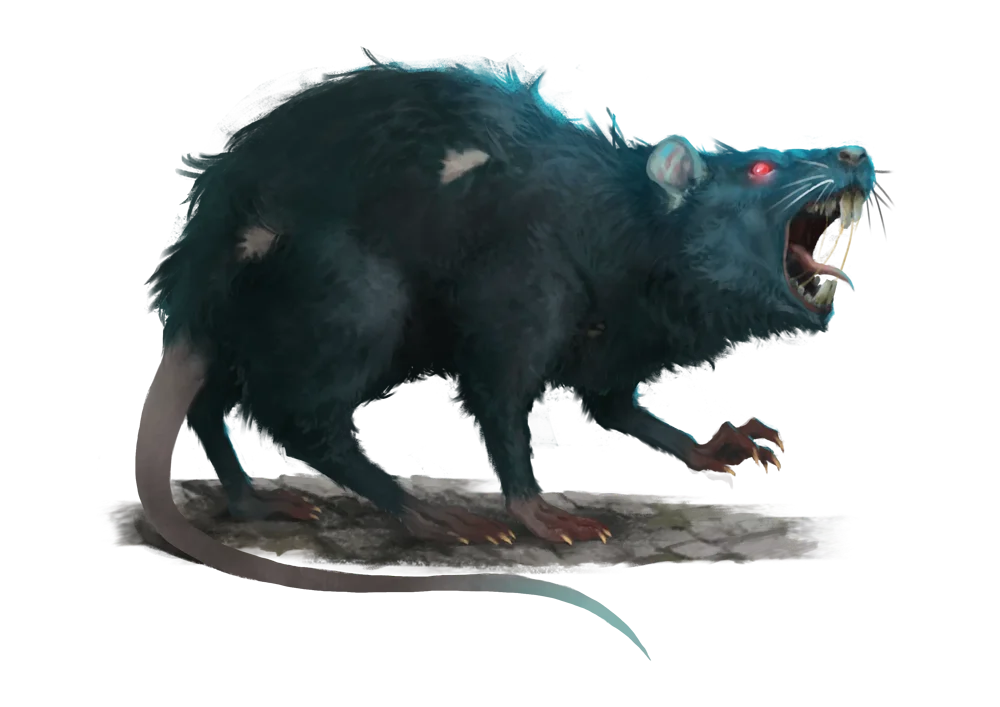
\includegraphics[width=3.2in]{book/img/Giant_Rat}
  \end{minipage}

  Double the amount of rats for the amount of PC's, and the rival group of monster hunters will join in the fight. This is a low-level threat to hook the players immediately into the context. The elder dives out of the way and when the PC's have cleared the rats with the help of their rivals, the elder will return and exhort them to go down into the well and find the source of the blight on their village.

  The PC's can either press the elder for another possible way into the well and he will explain he used to know of a cave by the water. Otherwise, they can go down the well itself.

  The rival group says they will have better luck up stream in the foothills, and take off to the North.

  Once down into the caverns beneath the village, the players will see that the water looks poisoned. If they cross the water to the East, they can find a treasure chest which is trapped. It is backed up against an old looking rotted wooden wall. If the players go around the wall through a side passage, they will see that the chest is wired into a trap and can disable the trap from that side. If they do not, and they try to open the chest, the trap will trigger which will be a Poisoned Lock.

  When they continue North through the cavern they will be confronted with more traps laid by the corrupted Swarm Voice ahead. There are four bear traps on the sides of the cavern which are wide enough to stand on. The PC's can either disarm two of these 4 traps to go further into the cavern, or they can get into the diseased water and wade through the center. If the PC's get into the water, they must make Fortitude saves against Scarlet Fever DC 13 Fortitude and gain sicked 1.

  Once they round the bend they will be greeted by a Corrupted Swarm Voice at level 3, who had deployed two more traps in this room, on the North and South sides. The Voice has two Tunnel Vipers in the room with him.

  When the fight begins, the rival group of monster hunters will emerge from the tunnel to the North and claim the battle to be theirs. As they move in, they will need to disarm the trap to the North and continue their way to the Voice.

  During the course of the battle, the Voice will make a corrupting call against the rival group and each one of them will succumb to the call. Their eyes will start glowing red with energy crackling from it like the Voice's, but they will shake it off one by one, and their eyes will return to normal.

  When they defeat the Voice and his Vipers, the PC's and the rivals will discover that the Voice has been poisoning the well with the source here: a corrupted crystal that glows with red energy. Before the rival group can take the crystal, they will begin coughing fits with their eyes beginning to glow red once more, and they will burst out of the cavern back the way they came to the North.

  \section{Wrap Up}
  The group goes back to town to report to the elder that the source of the poison is dealt with. The elder compensates them with gold for their service.

  They don't see any sign of the rival group or their ship when they row back to their ship. Sarlohmon, their aged wizard who is depleted after attempting to force the reality tear shut, is intrigued by the stone they have uncovered from this corruption. The stone itself is a part of a key of immense power which can summon the closest corrupted being. The crystal appears to have two more pieces before it is whole. He implores the adventurers to keep searching.

\end{multicols}